\documentclass[10pt]{book}
\usepackage{preference}
\newcommand\R{\ensuremath{\mathbb{R}}}
\usepackage{listings}
\usepackage[dvipsnames]{xcolor}
\usepackage{hyperref}
\usepackage{url}
\definecolor{codegreen}{rgb}{0,0.6,0}
\definecolor{codegray}{rgb}{0.5,0.5,0.5}
\definecolor{codepurple}{rgb}{0.58,0,0.82}
\definecolor{backcolour}{rgb}{0.95,0.95,0.92}

\lstdefinestyle{myStyle}{
    backgroundcolor=\color{backcolour},   
    commentstyle=\color{codegreen},
    keywordstyle=\color{magenta},
    numberstyle=\tiny\color{codegray},
    stringstyle=\color{codepurple},
    basicstyle=\ttfamily\footnotesize,
    breakatwhitespace=false,         
    breaklines=true,                 
    captionpos=b,                    
    keepspaces=true,                 
    numbers=left,                    
    numbersep=5pt,                  
    showspaces=false,                
    showstringspaces=false,
    showtabs=false,                  
    tabsize=2,
    extendedchars=\true
}

\lstset{style=myStyle}
\lstset{language=Python}

\begin{document}

\def\chap#1#2{\ \\ {\large\bf#1 \ | \ \tt\scshape#2} \par}

\ \vspace{-1cm}

{\bf
\ \\
\Large\centerline{\scshape Методы оптимизации, лекции}
}\normalsize

\section{О предмете}

Слова оптимизация просисходит от слова \textit{optimus} --- поиск наилучшего решения.

Чем эта дисциплина занимается?

Поиск минимума или максимума какой-либо функции.
$f(x) \to \min (\max)$.

Например, $f(x)$ -- стоимость, которую мы хотим минимизировать.

Обычно мы бдуем рассматривать функции, действующие из множества в числа, $f: A \to \R$.

Поиск решения задачи, где у нас оптимизируется несколько параметро -- многокритериальная оптимизация.

Во многокритериальную оптимизацию сильно углубляться мы не будем.

Методы математической оптимизации также называют математическим программированием (программмирование $\equiv$ поиск оптимального плана).


\subsection{Какиого вида может быть функция $f$?}

\subsubsection{Линейная}
Пусть $f(x) = \varphi \cdot x$.

Как правило, есть дополлнительные ограничения $A \cdot x = b$ ($A$ -- матрица, $b$ -- вектор).
$x_i \geqslant 0$.

\begin{example}[Транспортная задача]
    Есть $n$ складов, $m$ магазинов как эффективнее огранизовать логистику?
\end{example}

Вообще, бывают задачи, где ограничения есть и где их нет.

\subsubsection{Квадратичная функция}
Пусть $f(x) = \varphi \cdot x + x^T \cdot \theta \cdot x$.

Простоейшая задача -- линейная регрессия.
При помощи линейной функции покрыть множество точек, так чтобы сумма квадратов отклонений была минимальным.

Так как квадратичная функция выпукла, то ответ, обычно, бывает один.

В более сложных случаях глобавльных минимумов может не быть и придется искать локальные минимумы.

\subsubsection{Нельнейная функция}
$f(X) \to \min, f(X) \to \R$.
Иногда, функция может быть дискретной.
Например, в задачах динамического программирования.

\begin{example}
    Пусть есть окружность с радиусом $R$, нужно вписать в него прямоугольник со сторонами $a$ и $b$.

    $f = a \cdot b$.
    Ограничение $\sqrt{a^2 + b^2} = 2R$.
\end{example}

\begin{example}
    Обчуение различных моделей машинного обучения.
\end{example}


\subsection{Методы решения}
Иногда можно решить аналитически или в явном виде.

Но, это получается отнюдь не всегда.

\begin{definition}
[Итеррационные методы решения]
    Позволяют на каждом своем шаге как-то уточнять результаты решения.
    И таким образом можно получить, возможно, не точное решение, но достаточно близкое к нему.
\end{definition}

Пусть есть некоторая фунция $f: \R^n \to \R$.
Методы решения бывают детерминимрованными и стахастическими.

Один из методов решения -- \textbf{метод Монте-Карло} (генерируем случайные решения, проверяем, что они подходят, выбираем среди них оптимальный).
В этом методе надо вычислять только значние функции.

Еще один метод -- \textbf{метод иммитации отжига}.
Мы находимся в точке, выбираем еще одну точку.
Сморим, там значение меньше или больше в зависимости от этого получаем вроятность, что мы туда перейем.

Классификация методов по порядкам:
\begin{itemize}
    \item Нулевого порядка -- считаем только значние функции;
    \item Первого парядка -- используем градиенты изменения функции;
    \item Второго порядка -- используем вторые производные.
\end{itemize}

Еще один метод нулевого порядка -- \textbf{метод Нелдера -- Мида} (похоже на симпликс-метод, но для большего множества задач).

И еще один метод нулевого порядка -- \textbf{эволюционный метод или генетические алгоритмы}.
Использование подходов монте-карло с методами эволюции -- скрещеванием, матацией и отбором.

Методы \textbf{первого порядка} используют производные или градиенты.
Из математичсекого анализа известно, что градиент показывает направление наибольшего роста фнукции и, следуя туда, можно найти какой-то экстремум.

Самый простейший метод -- градиентный спуск.
Берем точку начального приближения, считаем в ней градиент и шагаем по направлению градиента.
Такой метод сходися.
На некоторых классах функции дает достаточно неплохой отевет.

Метод наискорейшего спуска.
Считаем градиент в одной точке и там, где в том направлении, где градиент минимальный.
Ищем в том направлении минимум и переходим туда.

В методах \textbf{второго порядка} используются матрица вторых производных -- гессиан.
Ингда читать вторые производные достаточно накладно.
Поэтому,  такие методы применяются достаточнно редко и для специфических задач с небольшим количством параметров.

Один из таких методов -- метод ньютона.

Есть \textbf{квази--ньютоновские методы}.
Они приближают матрицу вторых производных и это позволяет не считать матрицу явно.
BFGS.


\subsection{Почему Python?}
Python на данный момент является стандартом как для научного программирования, так и для, в частности, машинного обучения.

С одной сторны, питон очень простой.
С другой стороны, на питоне есть большое количество библиотек.

Да, Python очень медленный.
Однако есть библиотеки, например numpy, которые используют оптимальные оптимизации и засчет этого будет большой выигрыш.

\subsubsection{Библиотеки для python, без которых жить будет сложно}

\paragraph{NumPy} -- самая важная библиотека.
Позволяет работать с многомерными числовыми массивами и выполнять операции над ними.

Зачастую нужно будет сформулировать свой алгоритм так, чтобы он выражался в виде операций над массивами.

Оффициальный сайт \href{https://numpy.org/doc/stable}{numpy.org/doc/stable}.

\textbf{Broadcasting}.
В nympy особенное предобразование массивов.

Если умножить число на массив, число неявно превратится в массив и после этого произойдет поэлементное умножение.
То же самое есть с массивами разных размерностей.

\paragraph{SciPy}
Библиотека для научных вычислений на Python.
В ней есть много уже готовых алгоритмов, в том числе методов оптимизации.

Сайт \href{https://scipy.github.io}{scipy.github.io}.

\paragraph{MatPlotLib}
Библиотека для построения различных визуализаций, графиков и т.д.

Сайт \href{https://matplotlib.org/}{matplotlib.org}

\paragraph{Pandas}
Библиотека для работы с таблицами и табличными данными.

Сайт \href{https://pandas.pydata.org}{pandas.pydata.org}

\subsubsection{Как работать с python}
Есть такое понятие, на \textbf{jupiter notebook}.
Это интерактивные блокноты в которых можно писать на python или других языках,
писать текст с математическими формулами и делать раличные визулизации.

Редакторы можно использовать различные.
Можно писать в VS Code или PyCharm, еще есть Google Cloud.

\paragraph{Массивы в python}
\begin{lstlisting}
    a = [1, 2, 3, 4, 5, 6, 7, 8, 9]
    a[-1] # 9
    a[2:2] # [3, 4]
    a[::-1] # [9, 8, 7, 6, 5, 4, 3, 2, 2, 1]
\end{lstlisting}

\subsubsection{Испольщование numpy}
\begin{lstlisting}
    import numpy as np
    a = np.array([1, 2, 3, 4, 5, 6, 7, 8, 9])
    a * 2 # [2, 4, 6, 8, 10, 12, 14, 16, 18]
    [1, 2, 3] + [4, 5, 6] # [1, 2, 3, 4, 5, 6]
\end{lstlisting}

\begin{lstlisting}
    a = np.arrange(0, 10)
    a # array([0, 1, 2, 3, 4, 5, 6, 7, 8, 9])
    a + 10 # array([0, 1, 2, 3, 4, 5, 6, 7, 8, 9, 10])
    a ** 2 # array([0, 1, 4, 9, 16, 25, 36, 49, 64, 81])
    np.sin(a) # sin foreach elements
    np.sum(a) # sum of elements
    a[a > 3] # [4, 5, 6, 7, 8, 9]
    a.shape() # (10,)
    a.reshape(2, 5) # [[0, 1, 2, 3, 4], [5, 6, 7, 8, 9]]
    a.reshape(2, 5).T # [[0, 5], [1, 6], [2, 7], [3, 8], [4, 9]]
    a.reshape(2, 5) * [-1, 2] # [[0, 2], [2, 6], [4, 10], [6, 14], [8, 18]]

    b = np.array([[0, 1], [2, 3], [4, 5], [6, 7], [8, 9]])
    b[:, 0] # [0, 2, 4, 6, 8] -- first column
    b[0, :] # [0, 1] -- first line
    b[:2, :2] # [[0, 1, [2, 3]]

    np.array([1, 2, 3, 4, 5])[:, np.newaxis]
\end{lstlisting}

Графики
\begin{lstlisting}
    x = n.linspace(0, 10, 100)
    plt.plot(x, x) # graphic of f: [0, 10] to [0, 10], f(x) = x
    plt.plot(x, np.sin(x)) # graphic of f(x) = sin(x)

    x = n.linspace(0, 10, 1000)
    plt.plot(x, np.sin(x ** 2))
    plt.grid()
    plt.xlabel("axis x")
    plt.title("$\sin x\^2$")
\end{lstlisting}


\section{Градиентный спуск}
Пусть нам дана функция $f$. Найдем минимум функции.

Величина \textbf{learning rate} -- скорость обучения.
Сами итеррации можно назвать эпохами.

Градиентный спуск может быть стахастическим.
В этом случае градиент можно считать не целиком, выбирая только часть каких-то параметров.

Иногда можно иметь шаг не константный, а подбирать его каждый раз при помощи какого-то метода.

Градиент можно вычислять при помощи численных методов.
Например, через центральную разность

$h = \varepsilon$, $f_k^{\prime} (X) = \dfrac{f(X + h \cdot (0, \dots, 1_k, \dots, 0)) - f(X - h \cdot (0, \dots, 1_k, \dots, 0))}{2h}$.

Еще один важный вопрос -- масштабирование. Удобно искать решения, если расстояня при приближении по ращличным осям примерно равны. Хуже, когда есть вытянутые овраги.

Число обусловенности (condition number).
Абсолютное число обучловенности:
\[
    \lim_{\varepsilon \to 0} \sup_{\|\delta x \| \leqslant \varepsilon} \dfrac{\|\delta f(x)\|}{\| \delta x \|}.
\]


 
\subsection{Одномерные методы оптимизации}

Пусть у нас есть функция $f(x)$.

Пусть мы выбрали некоторое напроавление $p$.
Тогда для оптимизации мы можем рассматривать функцию
$\varphi(\alpha) = f(x_k+ \alpha p_k), \alpha > 0$.

\begin{center}
    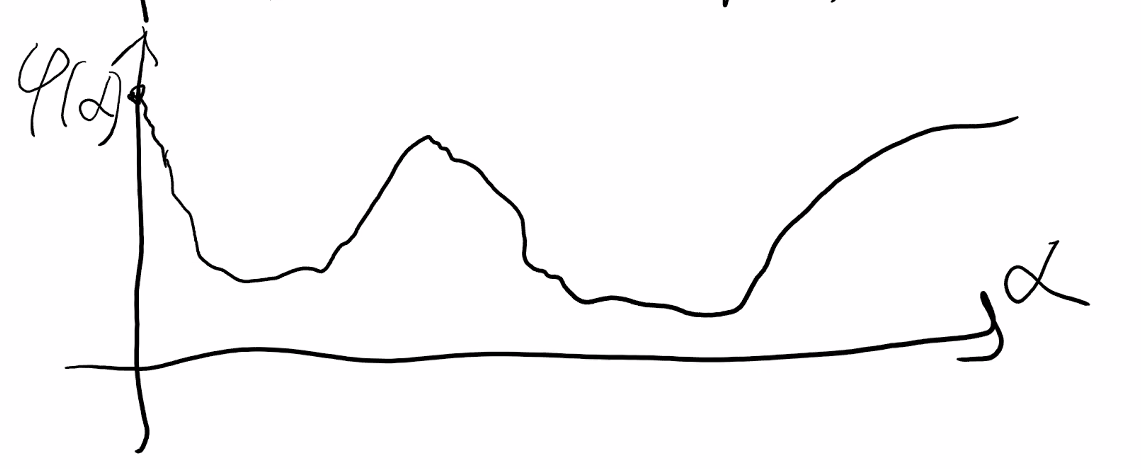
\includegraphics[scale=0.5]{img/methopt_one_dimensional_optimization_f_proect}
\end{center}

Наша задача~--- найти некоторый локальный минимум этой функции.

Встает два вопроса:
\begin{itemize}
    \item Как найти этот минимум?
    \item Как точно искать этот минимум?
\end{itemize}

Если вычислять очень точно, мы потратим очень много на это ресурсов.
Если искать не точно, есть риск потерять сходимость функции.

Какие бывают методы поиска локального минимума в этой задаче?

Пусть нам известна точка $x_k$, мы хотим найти еще две точки $x, y$, в одной из которых ($y$) функция будт меньше, а в другой ($z$), больше чем в той ($y$).

\begin{center}
    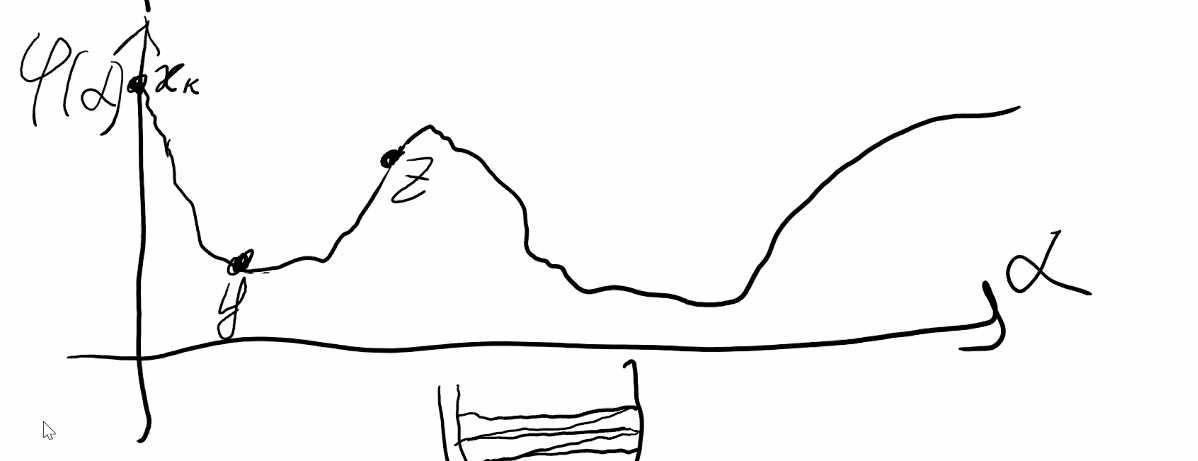
\includegraphics[scale=0.5]{img/methopt_one_dimensional_optimization_f_proect_points}
\end{center}

Как правило здесь используют довольно примитивные подходы.

У нас убывает функция, давайте возьмем некоторый шаг $\alpha$ (обчно $< 1$) и посчитаем $\varphi (\alpha)$.

Если там фунция меньше, чем $\varphi (0)$, то мы нашли $y$. Как найти $z$.
Давайте восколько-нибудь увеличим шаг $\alpha$, например, в два раза и посчитаем там $\varphi(2 \alpha)$.
Там может быть $\varphi(2 \alpha) > \varphi(\alpha)$, то $z = 2\alpha$.
Иначе, путь $y = 2\alpha$, а $z$ стоит попробовать найти еще раз.

Что делать, если $\varphi(\alpha) > \varphi(0)$.
Тогда возьмем $ \alpha / 2$ и попробуем сделать то же самое.

Допустим, мы нашли некоторый интервал, на котором есть минимум.
То есть есть три точки, в средней из которых функция меньше.
Один из способов дальшнейшего исслежования функции --- \textbf{метод дихатомии}.
Возьмем центр этого интервала и изучать поведение функции справа и слева от этой точки: $\varphi\left(\dfrac{a+b}{2} \pm h \right)$.
$h$ --- выбирается $\pm$ имперически.

\begin{center}
    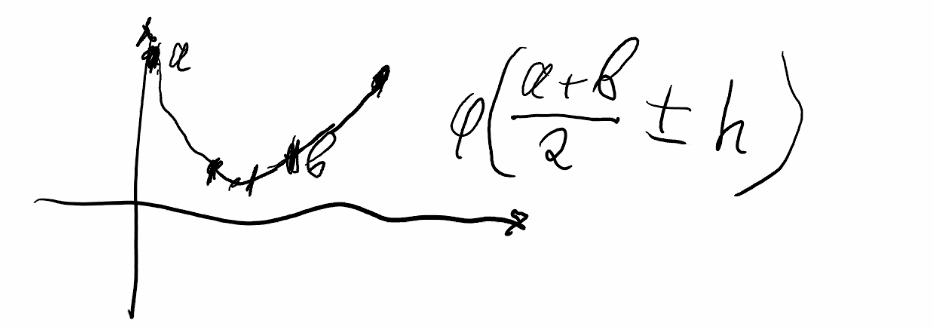
\includegraphics[scale=0.5]{img/methopt_one_dimensional_optimization_f_proect_pmh_points}
\end{center}

Дальше мы справниваем знаение функции слева и справа ($\pm h$) и переносим ближайшую крайнюю точку в точку с большим значением.
На рисунке выше мы перенесли $b$ в точку $\dfrac{a+b}{2}+h$.

Плюсы такого метода: простой метод (по модулю предположения, что функция унимодальна), считать просто.\\
Минусы: не очень сильно эффективен (на каждый шаг два вычисления функции).

Более эффективный метод: метод золотого сечения (метод Фибоначчи).

Еще один из простых, но при некоторых предположениях достаочно эффективный~--- \textbf{метод полиномиальной Аппроксимации}.
Предположим, что функция очень близка к какому-то полиному.
Самое просто~--- квадратичному полиному (параболе).

Пусть у нас есть три точки, проведем через них параболу.
Теперь аналичтически найдем точку минимума этой параболы и в этой точке посмотрим явное повдение нашей функции.

Дальше, так же, как в Дихатомии, сдвиним рассматриваемый отрезок фунции и повторим наши действия.

\begin{center}
    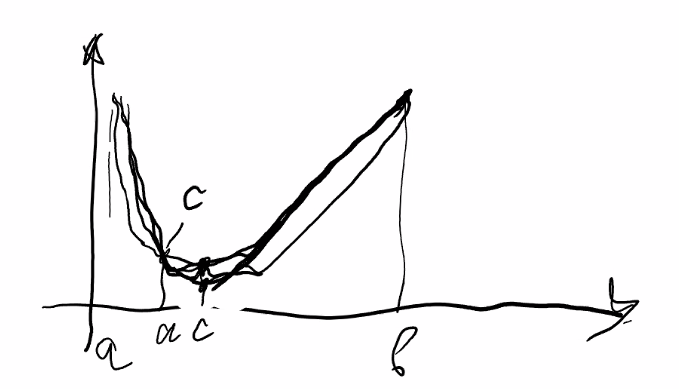
\includegraphics[scale=0.7]{img/methopt_one_dimensional_optimization_polynomial_approx}
\end{center}

Плюсы: если функция хорошая (достаточно гладкая, вблизи минимума хорошо аппроксимируется вблизи минимума).\\
Минусы: если функция плохая, будет работать очень не точно.

Еще можно аппроксимировать с использованием \textbf{производных}.
Пусть в точках $a$ и $b$ мы знаем не только значение $\varphi$, но и значение производной $\varphi^\prime$.

Для аппроксимации есть эрмитовы полиномы, их 4:
\begin{center}
    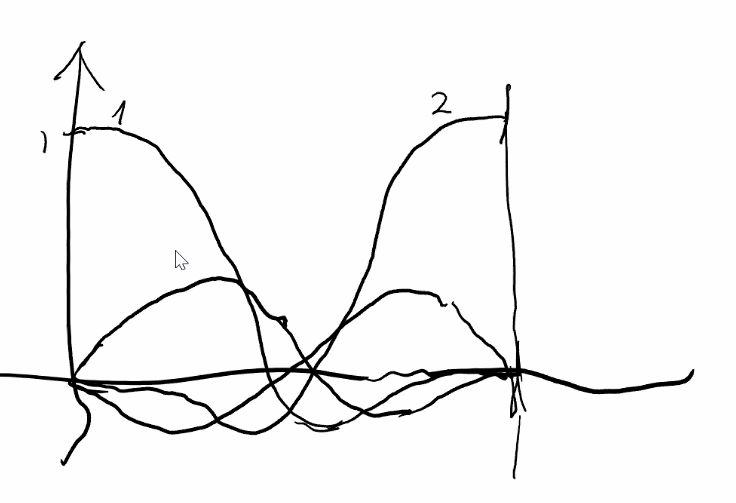
\includegraphics[scale=0.4]{img/methopt_one_dimensional_optimization_ermyt_polynom}
\end{center}

Возьмем:
$\varphi(a) E_1 + \varphi (b) E_2 + \varphi^\prime (a) E_3 + \varphi^\prime (b) E_4$.

Плюсы и минусы те же.
Кроме того, функция $\varphi$ должна быть достаточно гладкой, что бы мы могли вычисялять ее производные.

\textbf{Метод Ньютона} (метод касательных).
Строим касательные (производные), ищем их пересеченеи с нулем ($\varphi^\prime = 0$).
Найденные точки (нули) и есть ответ.

Плюсы: если функция квадратичная (или другая хорошая) будет очень быстро сходиться.\\
Минусы: нужны вторые производные.

\textbf{Метод секущих (хорд)}.
Так же, как в методе Ньютона, ищем нули.

\subsubsection{Условия Вольфе}

Условия выбора следующей точки для исследования ее на минимум.

\begin{enumerate}
    \item $f(x_k + \alpha p_k) \leqslant f(x_k) + c_1 \alpha \triangledown f (x_k) p_k$,\\
    где $0 < c_1 < 1$, $c_1 = 10^{-4}$.
    \item $\triangledown f(x_k + \alpha_k p_k) \cdot p_k \geqslant c_2 \triangledown f(x_k) \cdot p_k$.
\end{enumerate}

Первое условие накладывает вограничения на выбираемое $\alpha$.
\begin{center}
    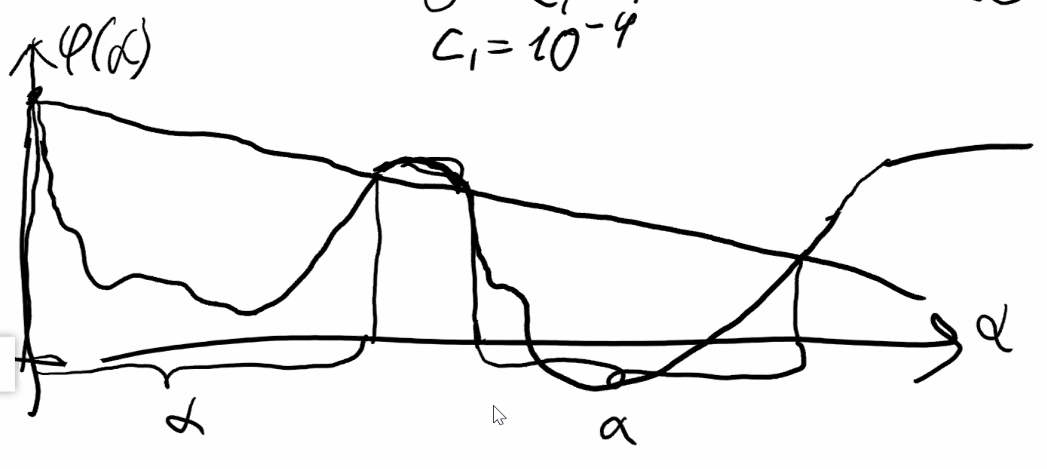
\includegraphics[scale=0.4]{img/methopt_volfe_conditions_1}
\end{center}

Первого условия не достаточно, так как можно взять $\alpha = \varepsilon$ и это условие там будет выполняться. \\
Второе условие заперщает делать делать слишком маленькие шаги и шагать туда, где градиент продолжает достаточно быстро убывать

\begin{center}
    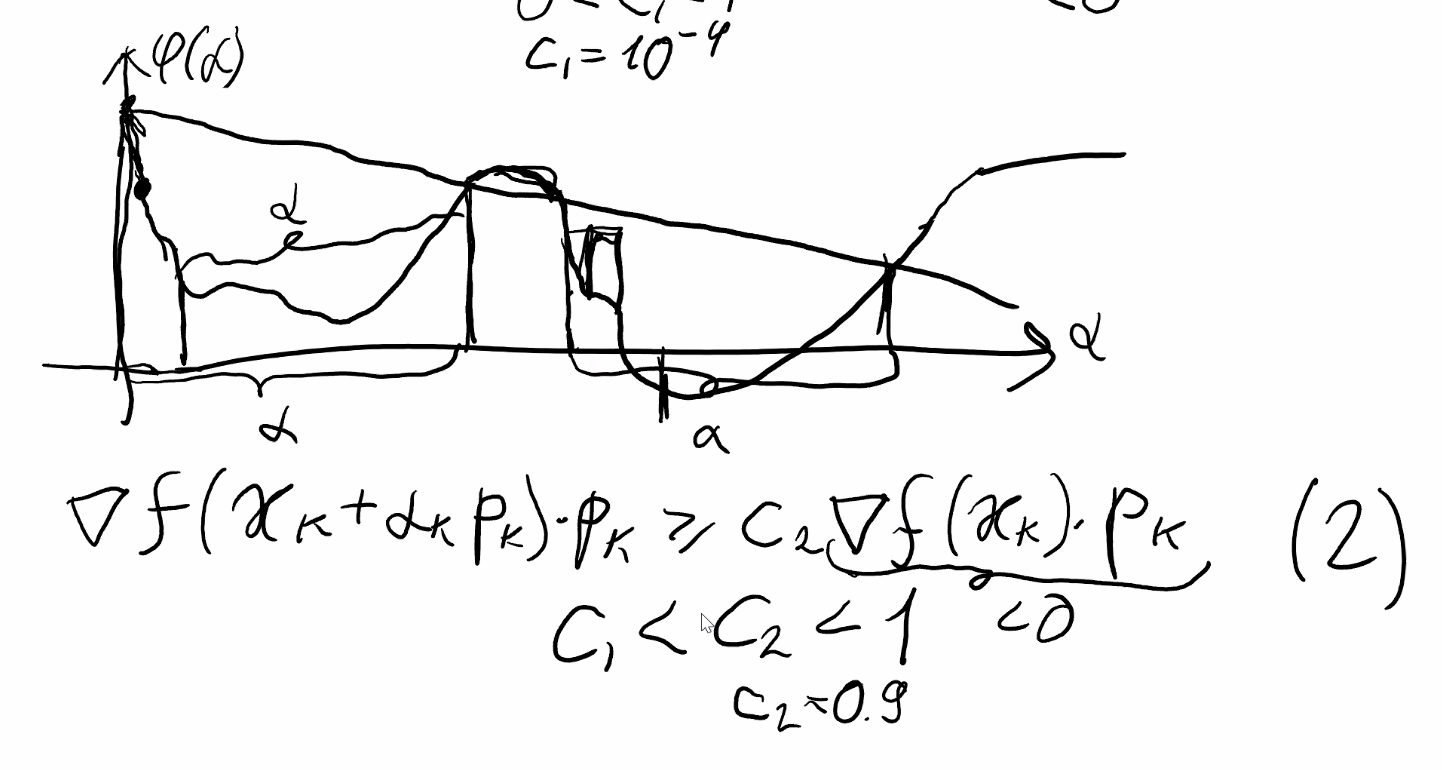
\includegraphics[scale=0.333]{img/methopt_volfe_conditions_2}
\end{center}


    Одномерная оптимизация~--- некоторый итерративный процесс, в котором мы ищем некоторый локальный минимум и потом пытаемся его улучшить. Возникает вопрос, а в какой момент нужно остановиться?
    Мы можем добиваться точности один знак после запятой или десять знаков после запятой. И так и так, мы можем в итоге прийти к минимуму многомерной функции.

    Ответ на возникший вопрос~--- условия Вольфе. Как только они стали выполняться, мы можем прикрать одномерную опитимизацию.

Вспомним условия Вольфе:
\begin{enumerate}
    \item $f(x_k + \alpha p_k) \leqslant f(x_k) + c_1 \alpha \triangledown f (x_k) p_k$,
    \item $\triangledown f(c_k + \alpha_k p_k) \cdot p_k \geqslant c_2 \triangledown f(x_k) \cdot p_k$.
\end{enumerate}
Где, $c_1, c_2$~--- некоторые параметры, удовлетворяющие условию     $0 < c_1 < c_2 < 1$.

\begin{proof}[Доказательство корректности условий Вольфе]
    Запишем правую часть первого условия в виде функции и получим прямую, которая идет из начальной точки $x_k$ и убвает. В некоторой точке $\alpha^\prime$ она пересекается с функцией. Для $a^\prime$ верно $f(x_k + \alpha^{\prime} p_k) = f(x_k) +\alpha^\prime c_1 \triangledown f(x_k) \cdot p_k)$.

\begin{center}
    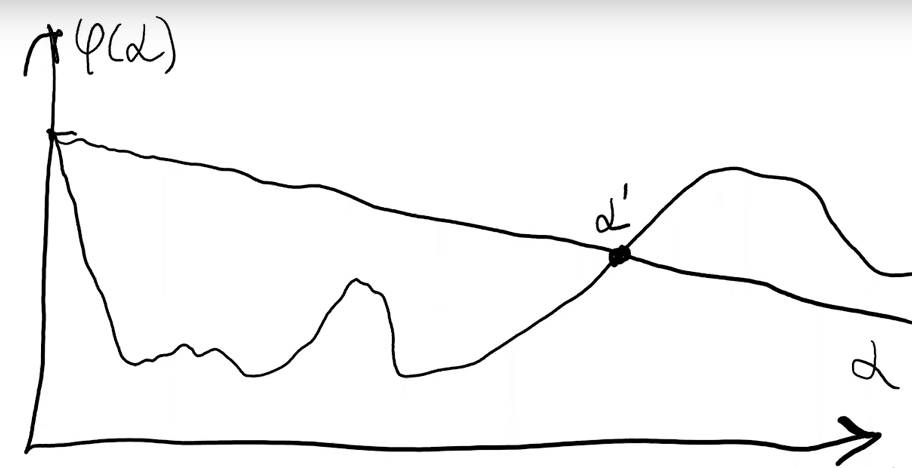
\includegraphics[scale=0.4]{img/methopt_volfe_conditions_proof}
\end{center}
    Заметим, что первое условие выполнятется всюду, где $\alpha < \alpha^\prime$.
    Почему где-то на этом интервале выполнится второе условие?
    
    \[f(x_k  + \alpha^\prime p_k) - f(x_k) = \alpha^\prime \triangledown f(p_k +\alpha^{\prime\prime} p_k) p_k, ~~~ \text{где } \alpha^{\prime\prime} ~\text{ --- некоторая неизвестная нам точка}. \]
    Тогда,
    \[ \triangledown f(x_k + \alpha^{\prime\prime} p_k) \cdot p_k = c_1 \triangledown f(x_k) \cdot p_k > c_2 \triangledown f (x_k) p_k. \]
    Таким образом, $\alpha^{\prime\prime}$ удовлетворяет второму условию Вольфе.
\end{proof}

Введем обозначение $\cos \Theta = \dfrac{-\triangledown f(c_k) \cdot p_k}{\| \triangledown f(x_k) \| \|p_k\}}$.

\begin{theorem}
    Если $p_k$~--- направление поиска, $\alpha_k$ удовлетворяет условиям Вольфе,
    $f$ огра\-ни\-че\-на и непрерывно дифференцируема и градиент функции $f$ является Липшица--непрерыным ($\| \triangledown f - \triangledown f(\overline{x}) \| \leqslant L \| x - \overline{x} \|$, ~$L > 0$). Тогда будет выполняться следующее соотношение 
    \[\sum_{k\geqslant 0} \cos^2 \Theta_k \| \triangledown f(x_k)\|^2 < +\infty. \]
\end{theorem}
\begin{remark}
    Если $\cos^2 > 0$, то последовательность градиентов должна стремится к 0.
\end{remark}
\begin{proof}
    \[\underbrace{\left( \triangledown f(x_{k + 1}) - \triangledown f(x_k) \right) \cdot p_k}_{\leqslant \alpha_k L \| p_k\| ^2} \geqslant (c_2 - 1) \cdot \triangledown f(x_k) \cdot p_k. \]
    Выразим $\alpha_k$:
    \[\alpha_k \geqslant \dfrac{c_2 - 1}{L} \cdot \dfrac{\triangledown f(x_k) \cdot p_k}{\| p_k \|^2}.\]
    Скомбинируем условие на $\alpha$ с первым условием:
    \[f(x_k) \leqslant f(x_k) - \underbrace{c_1 \dfrac{1 - c_2}{L} \cdot \dfrac{\left( \triangledown f(x_k) \cdot p_k \right)^2}{\|p_k \|^2} }_{-c \cos^2 \Theta \cdot \| \triangledown f(x_k) \| ^2, ~~c = \frac{c_1 (1 - c_2))}{L}}
    \implies
    f(x_{k+1}) \leqslant f(x_0) - c \sum_{j = 0}^k \cos^2 \Theta \| \triangledown f(x_j) \|^2.\]
    Так как фукция была огранчиена, то ряд ограничен и сходится.
\end{proof}

\subsection{Стахастический градентный спуск}
\begin{problem}[Линейная регрессия]
    Пусть у нас есть некоторые точки на плоскости. Мы хотим провести некоторую прямую, чтобы минимизировать сумму квадратов отклонений.

    \begin{center}
        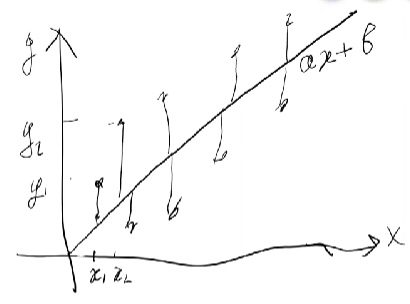
\includegraphics[scale=0.5]{img/linear_regression_problem}
    \end{center}

    Пусть есть функция $f(a, b) = \sum_{i=1}^n \left( a x_i + b - y_i \right)^2$. Хотим найти такие $a, b$, что $f$ принемает минимальное значние.

    Вообще, задачу можно решить аналитически.

    Но если обощить ее  на пространство более высокой размерности, аналитиечски решать будет сложно, численные методы лучше.

    Можно переформулировать задачу в матричном виде:
    \[Y = \begin{pmatrix}
        y_1\\ y_2\\ \dots\\ y_n 
    \end{pmatrix}, ~~~X = \begin{pmatrix}
        x_{1,1} & \dots & x_{1,n}\\
        \dots & \dots & \dots\\
        x_{n,1} & \dots & x_{n,n}.
    \end{pmatrix}, ~~~
    f = \| X \beta - Y \| ^2 \implies
    \beta = \left( X^T X \right) ^{-1} X ^T Y.\]

    Если размерность большая, это не сработает.
\end{problem}

\begin{definition}
    Пусть $f(x) = \sum\limits_j Q_j (x)$.

    Стахастический градиентный спуск заключается в выборе одного случайного слогаемого в сумме, вычислении градиента этого слогаемого и спуск по этому градиенту.
\end{definition}

\begin{itemize}
    \item[+] Один шаг очень дешевый.
    \item[-~] Результат от одного шага достаточно сомнительный,  поэтому говорить о сходимости данного метода не приходится.
    \item[-~] Найти точный минимум очнеь сложно.
\end{itemize}

У данного метода есть достаточно много модификаций.

Одна из наиболее популярных модификаций~--- \textbf{Mini Batch Gradient Descent}.
\subsubsection{Mini Batch Gradient Descent}
Мы можем проводить полный градиентный спуск, то есть считать граент по всем $n$ слогаемым (тяжело вычислять). Можем проводить стахастичесий градиентный спуск и считать градиен по одному слогаемому (получается не точно). А можем выбрать, например $10$ случайных слогаемых и посчитать по ним градиент.

В machine learning обыно выбирают не случайные слогаемые, а спрева перемешивают, а затем последовательно рассматривают первые $k$, вторые $k$ и т.д. слогаемых.

\end{document}